% Setup - do not change
\documentclass[11pt]{article}
\usepackage[top=0.9in, left=0.9in, bottom=0.9in, right=0.9in]{geometry} 
\usepackage{parskip}

\usepackage[english]{babel}
\usepackage[utf8]{inputenc}
\usepackage{amsmath,amsthm,amssymb,graphicx,pdfpages,lipsum,hyperref}
\usepackage[none]{hyphenat}
\usepackage{csquotes}
\usepackage{multicol}
\usepackage{subcaption}

\setlength\parindent{0pt}
%%%%%%%%%%%%%%%%%%%%%%%%%%%%%%%%%%%%%%%%%%%%%%%%%%%%%%%%%%%%%%%%%%%
% add other packages here if required

%% Bibliography are specified in this file. You can also choose inline bib style if you want to. But make sure your citation style is consistent (and proper)
% For more details on citation: https://library.unimelb.edu.au/recite
\usepackage[sorting = none]{biblatex}
\addbibresource{references.bib}

%%%%%%%%%%%%%%%%%%%%%%%%%%%%%%%%%%%%%%%%%%%%%%%%%%%%%%%%%%%%%%%%%%% the '%' symbol denotes comments

% Begin document creation
% DELETE THE \lipsum PLACEHOLDERS WHEN YOU BEGIN
\title{\textbf{Predicting Demand for Yellow Taxis in NYC} \\ Analyzing the Impact of Events and Weather}
\author{
Saleha Khalid \\
Student ID: 1122166 \\
%% Replace the link with your github repo
% 1. Remember to escape underscore (\_) in the link.
% 2. Remember to include the commit you want to submit in the link
\href{https://github.com/MAST30034-AppliedDataScience/project-1-individual-salehak/commit/eedf6e0d12d302930bc589b1683d2986f6cee033}{Github repo with commit}
}

\begin{document}
\maketitle

\section{Introduction}
With all the changes in the economy after the effect of COVID-19, are we actually on the road to recovery? The widespread lockdowns from COVID affected everything, from people’s mental health to financial security.\cite{covid19effects} The taxi business was also deeply affected as people had nowhere to go. As life returns to a semblance of normalcy, people are eager to return to their pre-COVID lives, leading to an increased demand for taxis as they attend more events and places. This study aims to analyze whether the events happening in New York City influence the demand for taxis. 

For this study and forecasting the demand required, I will be looking at two different Machine Learning methods and evaluating them to see if the hourly demand can be predicted for various regions in New York City (NYC) based on the weather for the day and permitted events for that location.

By doing so, taxi companies can be better prepared for these events, optimizing the number of taxis available to meet demand, thereby maximizing profits and reducing idle time on waiting to find other passengers.

\subsection{Dataset}
As mentioned previously, to look into the demand for yellow taxis, the primary dataset of choice for this project was the Yellow Taxi Trip Records, published by TLC (New York City Taxi \& Limousine Commission).\cite{nyctaxidata} These records contained information about the trips taken on yellow taxis, including pickup and dropoff times and locations, in addition to other information related to fares and tips. 

To make the predictions for the current year, I decided to look at the data for the previous year as it is assumed to be closest to matching the demand. Therefore, the data was extracted from January 2023 to April 2024. Another presumption was that going back any further from 2023, we would risk having effects from COVID-19 that we would not be able to account for.

As for one of the external datasets, I decided to use the NYC Permitted events dataset, which was taken from NYC Open Data, and then queried to retain only the events in the scope of the dates.\cite{nyceventsdata} This dataset contained several features about the events, such as the start and end time for that event, its name, location, type, and organizer. 

The second external dataset I used was the land surface climate for Central Park in NYC, published by the National Centers for Environmental Information.\cite{nceidailydata}This dataset provided us with information relating to daily climate with features such as temperature, relative humidity, wind speed, etc.


\section{Preprocessing}

\subsection{Yellow Taxi Dataset}
For the yellow taxi dataset, there were a total of 83,100,468 rows in the beginning, which were then processed using the following steps so that we only took records of the valid and necessary taxi trips.
The following criteria were followed to make sure that the data was within valid bounds as set up by the TLC\cite{nyctaxidatadictionary}:
\begin{itemize}
    \item Removed any rows which had categorical values not within specified values such as the Vendor ID, Rate Code ID, payment type, and the Location ID
    \item Kept only the rows where the numerical variables were valid, such as the following:
    \begin{itemize}
        \item Chose the fare amount to be greater than \$3 since that is the starting fare on the meter\cite{nyctaxifares}
        \item Trip distance had to be at least 0.4 miles since distances below that value are considered walkable
        \item Negative values were removed from the columns containing tax amount, tip amount, tolls amount, improvement surcharge, extra, and congestion surcharge, as these cannot logically be negative
    \end{itemize}
    \item The pickup and dropoff dates and times were filtered as well to keep the data where the trips were within the scope of defined set time
    \item For passenger count, we decided to keep at least one passenger (for it to be a valid trip) until a maximum of six passengers, as suggested on the NYC taxi official website.\cite{nyctaxifares}
    \item The total duration of the trips was calculated based on pickup and dropoff time, and only the negative values were filtered out
    \item Any extreme values from the tip amounts, fare amounts, trip distance, and duration were also removed as they would not give us an accurate representation of the typical trips
\end{itemize}

Only some columns were retained for this dataset, such as the pickup and drop off times and the pickup and drop off locations. Retention of those columns is mainly due to wanting to model for the demand in taxis which is not affected by the fares and tips. 

Although we only kept a few columns for this data, it was necessary to do all the previous steps in preprocessing for taking the valid taxi rides/trips into account. Trips to and from the airports were removed to prevent potential skewing of results, given that demand is typically strongest for these locations and is unlikely to be influenced by the events. These preprocessing steps left us with 64,344,743 rows and we retained around 77\% of the original data.

\subsection{Events Dataset}
Initially, the data consisted of 4,841,354 rows and 12 features, including the start and end date and time of the event, along with the location, which are the key features in this case. The primary issue with this data was the large number of duplicates, which were removed as a priority.
Next, the following steps were done as part of the preprocessing:
\begin{itemize}
    \item Removed events that are not likely to affect taxi demand, which included events such as closures, maintenance, parking, etc.
    \item Removed the features I believed would not be necessary, such as street closure type, community board, and whether the event is street side – the main idea is to only focus on the sheer volume of events in the area in hopes that it helps us determine the demand in taxis
    \item Since the data only provided us with the start time and end time of an event, I decided to combine the two features to give me a cumulative count of the events being run from start to end to get a better view of the number of events happening in a day at a specific time instead of having to model the two separately.
    \item As some of the events in the records contained several precincts, I decided to preserve that information. Those records were split into several rows based on the precincts to get a better understanding of the count of events for a specific location.
\end{itemize}
After all the preprocessing steps, the dataset was left with only 288,411 rows, which was about 5.95\% of the original data due to the sheer volume of duplicates.
From this data, I calculated aggregates for the number of events per hour for the different precincts to aid in the modeling process.


\subsection{Weather Dataset}
\label{subsec:weather}
An assumption was that the weather around New York City would be similar to the data captured for Central Park, so that was the only dataset exported for the weather. 
Initially, the dataset consisted of 56,833 instances and 123 features, excluding the date. Most of those were excessive, and we decided to keep 9 of those features.
\begin{multicols}{3}
\begin{itemize}
    \item Precipitation (in mm)
    \item Snowfall (in mm)
    \item Max. Temperature
    \item Min. Temperature
    \item Wind Speed
    \item Relative Humidity
    \item Fog
    \item Heavy fog
    \item Thunder
\end{itemize}
\end{multicols}
I also created another feature, the average temperature for the day, calculated from the minimum and maximum temperature. 
Some of the other steps I took for the preprocessing of the weather dataset are as follows:

\begin{itemize}
    \item Filtered the dataset for the dates in the scope of the study
    \item A couple of features, average wind speed and average relative humidity, had null values for the day. For those, I decided to take the average of the dates close to it that had values recorded. This is assumed to be relatively accurate considering weather data doesn’t vary significantly from day to day.
\end{itemize}
After all the preprocessing steps to the weather dataset, we were left with 486 instances and 10 features, retaining only about 0.9\% of the data, mainly due to the extreme volumes of data from the previous years, which were not needed for the study.

\subsection{Mapping Taxi Zones to Precincts}
Some other steps I decided to take for the events and taxi dataset is to try and map the taxi zones to the police precinct since the taxi data consisted of taxi zones for the location ID and the events dataset consisted of precincts for the location as well as boroughs, so I decided that having a more common ground for the comparison of the two would be significantly helpful in getting a better understanding.

\section{Analysis and Geospatial Visualization}
\subsection{Distribution of Taxi Pickups and Dropoffs in NYC}
\label{subsec:distribution}
From aggregating the data, I found that most of the taxi ride pickups were either around the Manhattan area, with some focused around Brooklyn and Queens because I decided to remove any trips to and from the airport since that was something I didn’t want to influence the other predictions and forecasts. The least pickups were around the Staten Island borough. 
The main reason for most of the taxi pickups and dropoffs being in Manhattan is probably because of high commercial activity and tourist attractions like Times Square. Similarly, Manhattan is known to be the center for many businesses. Staten Island, in contrast, has the least trips (both pickups and dropoffs) which is likely due to being less populated. The average pickups and dropoffs for the different boroughs can be seen in the Figure \ref{fig:comparison}.

\begin{figure}[h!]
    \centering
    \begin{subfigure}[b]{0.45\textwidth}
        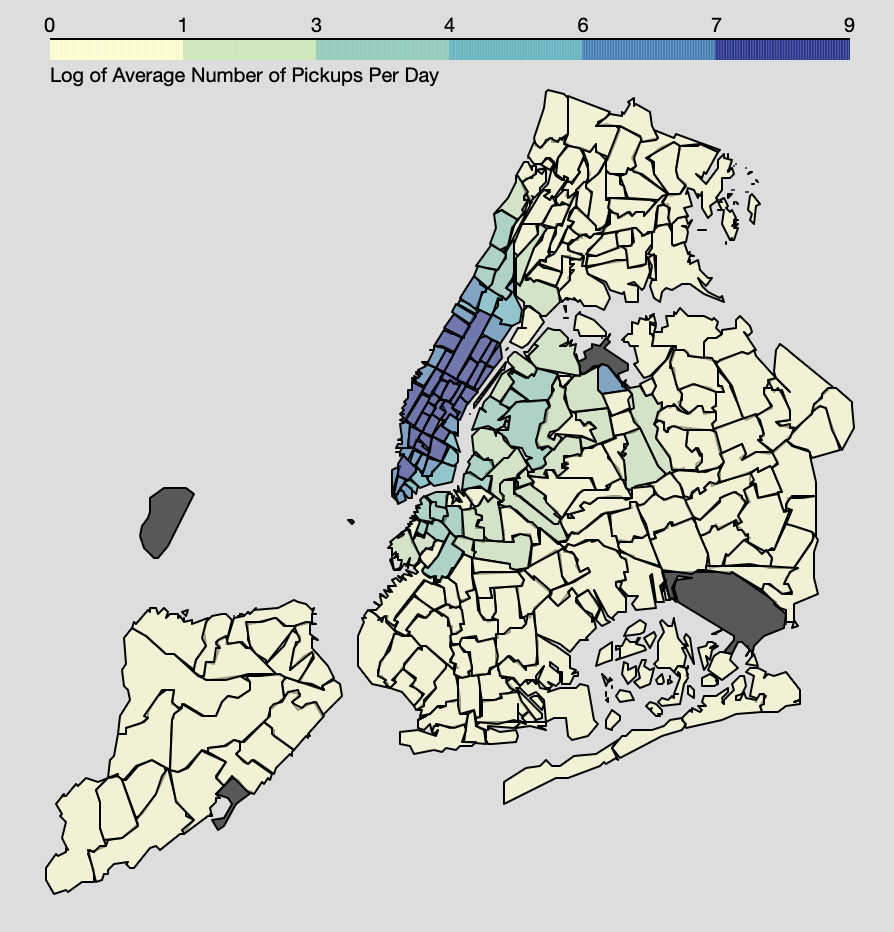
\includegraphics[width=\textwidth]{plots/LogAvgPU.png}
        \caption{Log of Average Number of Pickups Per Day}
        \label{fig:pickups}
    \end{subfigure}
    \hfill
    \begin{subfigure}[b]{0.45\textwidth}
        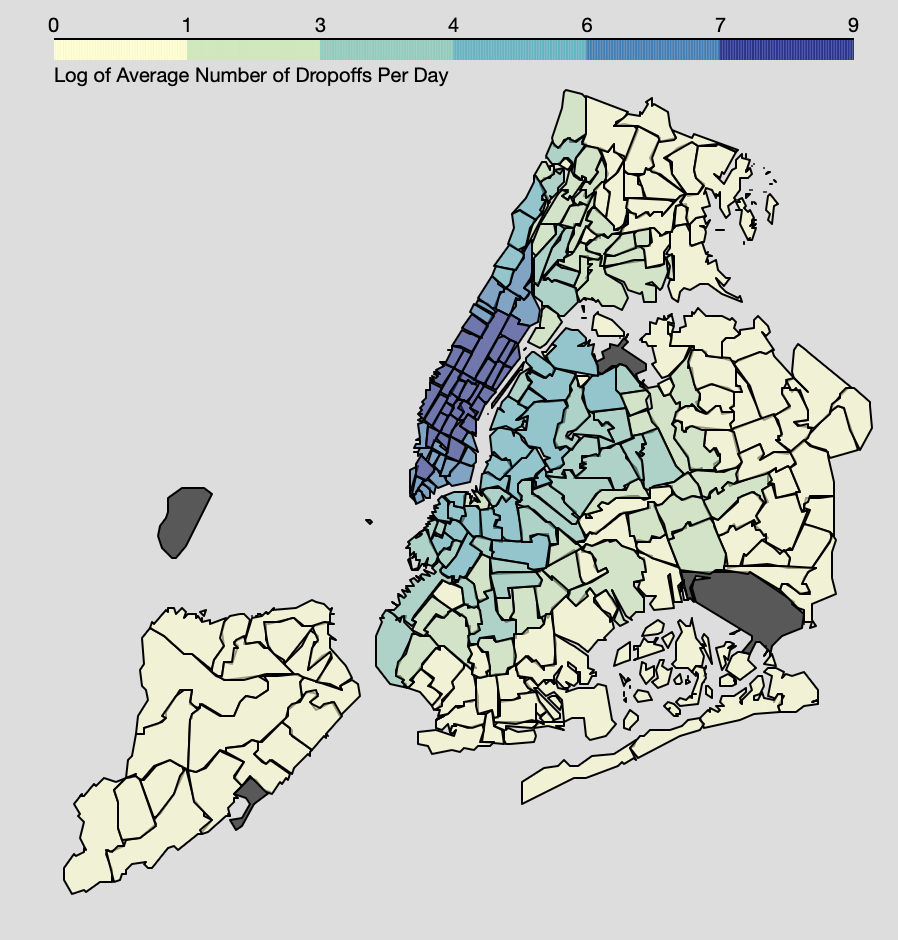
\includegraphics[width=\textwidth]{plots/LogAvgDO.png}
        \caption{Log of Average Number of Dropoffs Per Day}
        \label{fig:dropoffs}
    \end{subfigure}
    \caption{Comparison of Taxi Pickups and Dropoffs in NYC}
    \label{fig:comparison}
\end{figure}

\subsection{Distribution of Events in NYC}
Similar to the taxi data, from the events data, I found that most of the events were focused around the Manhattan area. It seems like the place to be for taxi pickups and events in New York City. This can be seen through the bar graph in Figure \ref{fig:events}, which shows the distribution of the total number of events in each borough. 

\begin{figure}[h]
    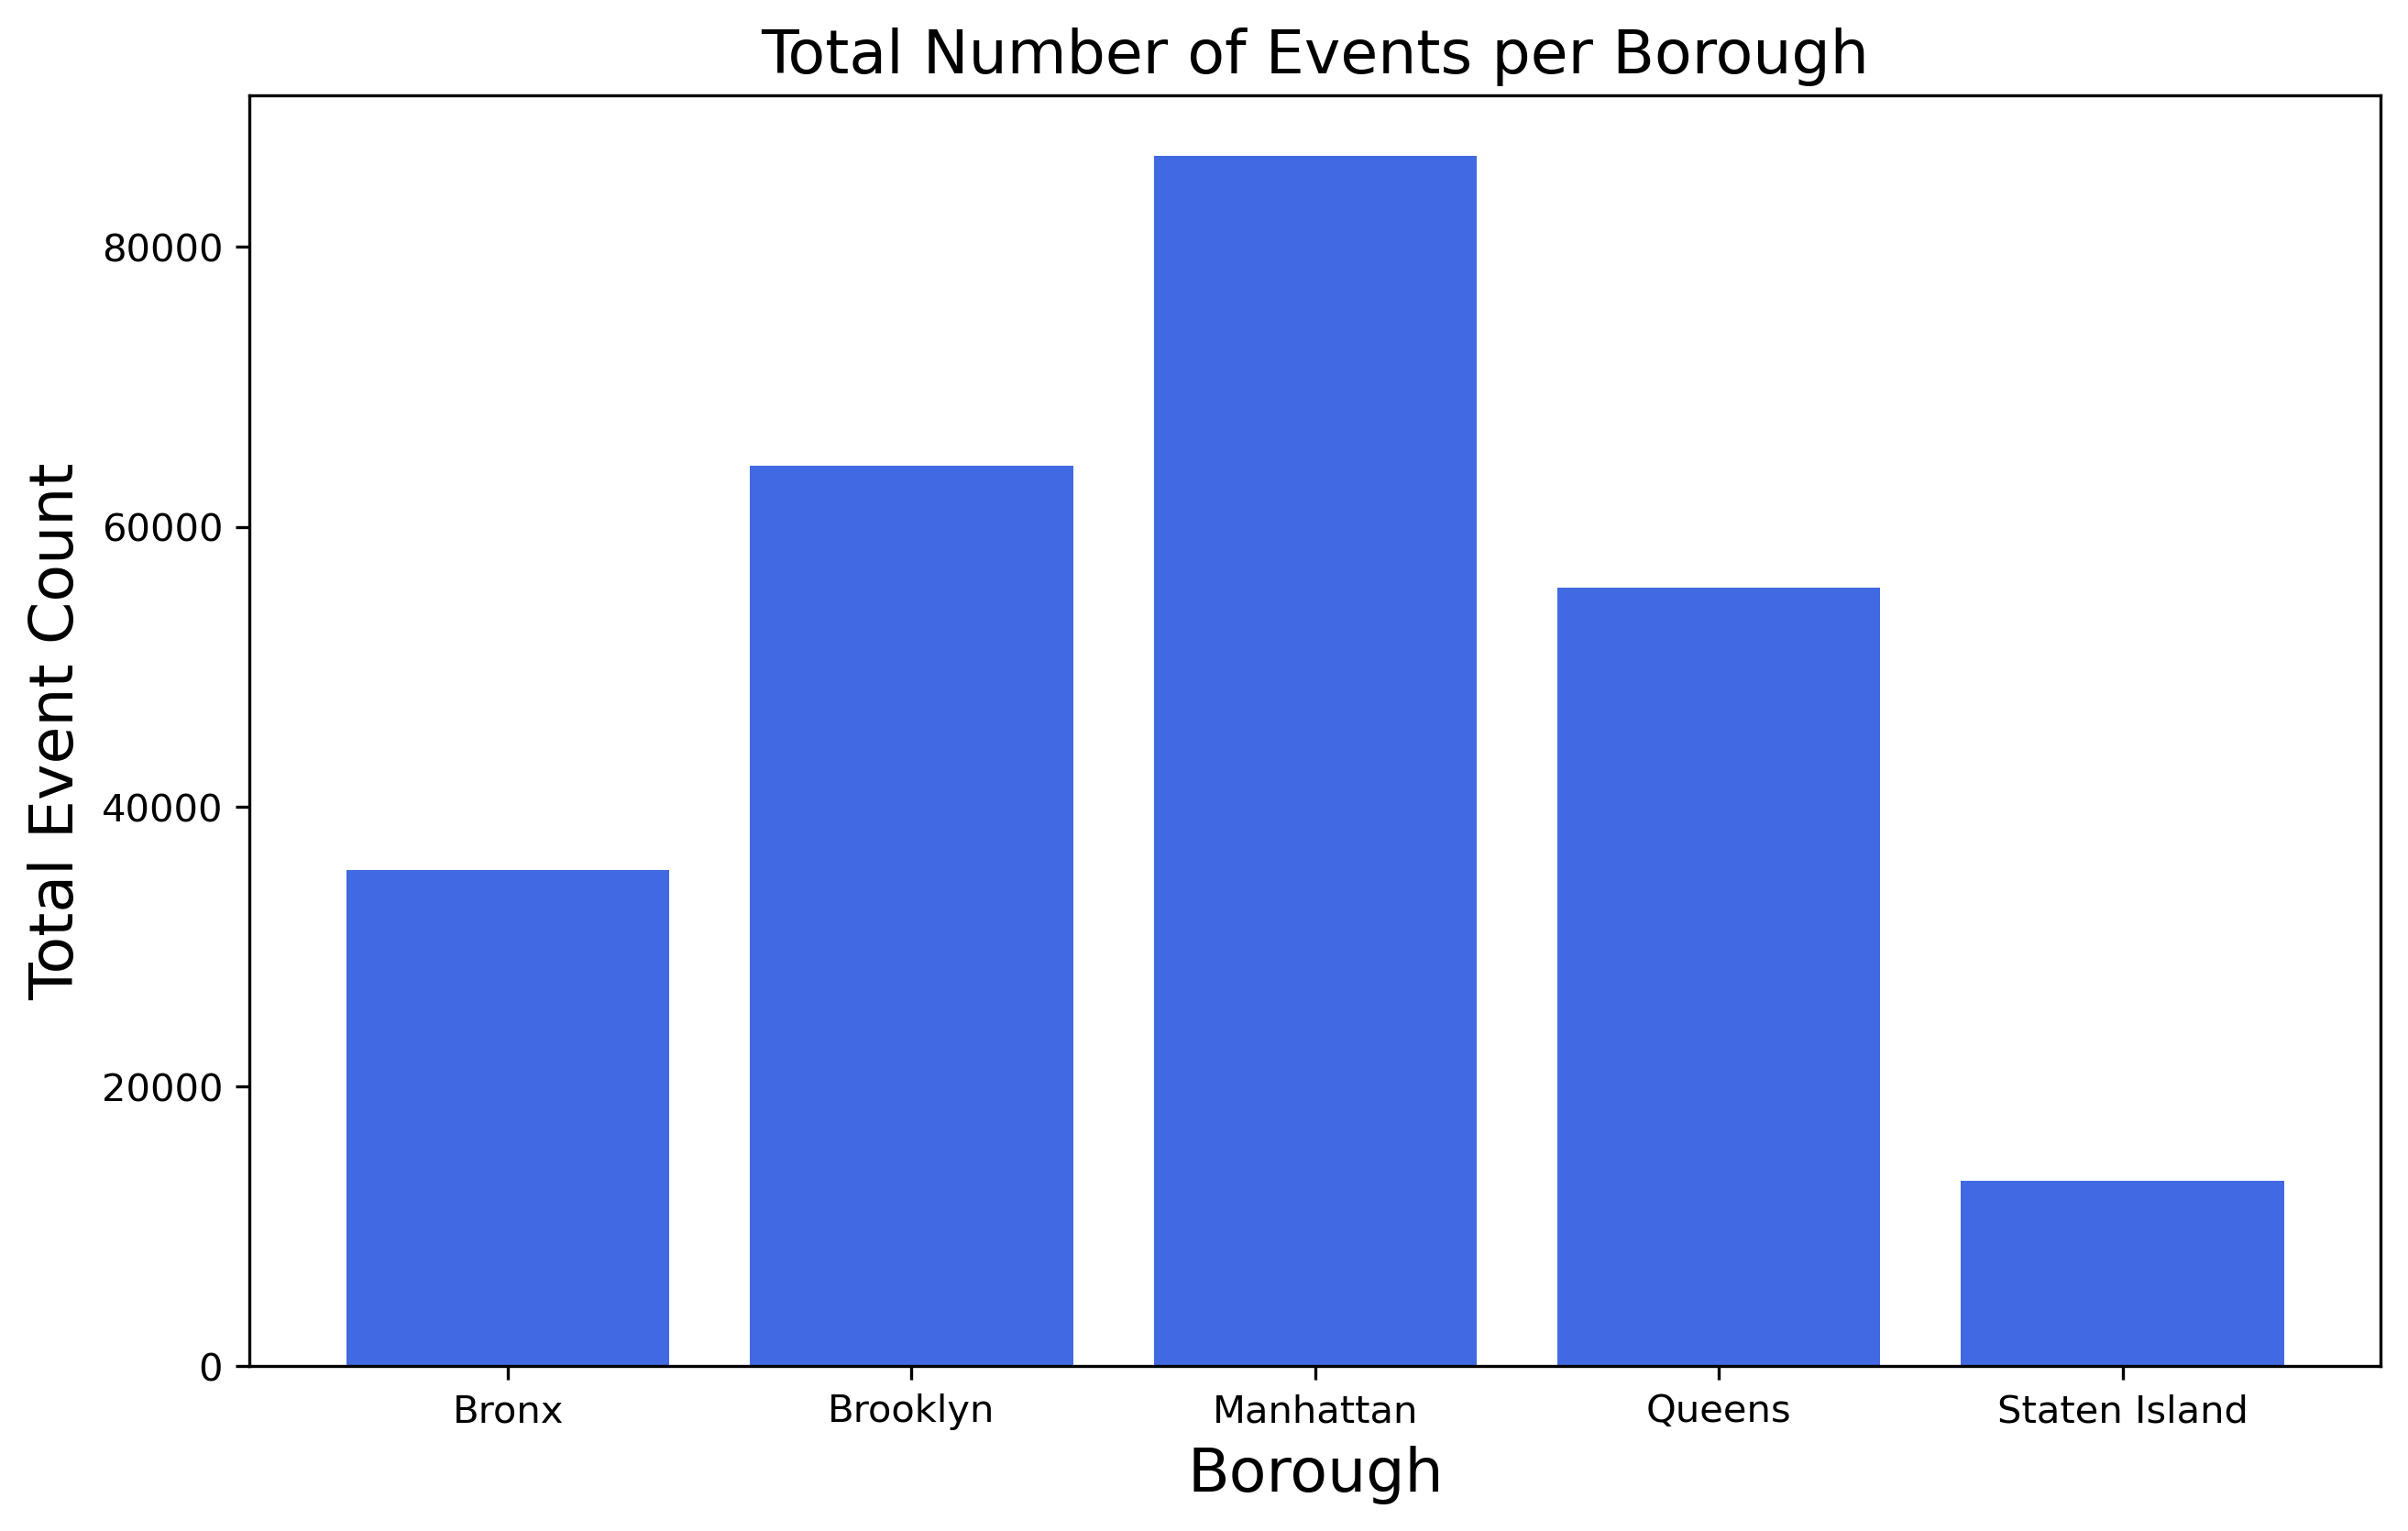
\includegraphics[width=0.5\textwidth]{plots/total_events_per_borough.png}
    \centering
    \caption{Total Number of Events per Borough}
    \label{fig:events}
\end{figure}

As seen in Section \ref{subsec:distribution}, taxi pickups and dropoffs, the distribution of events according to the boroughs is about the same as we would expect, with most of the events in Manhattan and some of the majority events being in Brooklyn and Queens, with the fewest in Staten Island.

\subsection{Trend of Hourly Events and Taxi Pickups}
For a better understanding of how the number of events in a day may affect the taxi rides, I decided to overlay the distributions of the average number of pickups daily and the average number of events being held daily on each other, as seen in Figure \ref{fig:events_vs_pickups}. The figure shows that the fewest events are from 11 pm to around 7 am, and the fewest taxi rides are from 4 am to 5 am. However, there is a steady incline for both events and pickups daily from around 9 am to 6 pm, with both peaks at 6 pm.
The graph in Figure \ref{fig:events_vs_pickups} also shows a clear peak in taxi demand from around 4 pm to 7 pm, which marks the end of the work day and the beginning of evening social events. From this, we know that commuter traffic and event attendance can drive taxi demand for those hours.

\begin{figure}[h]
    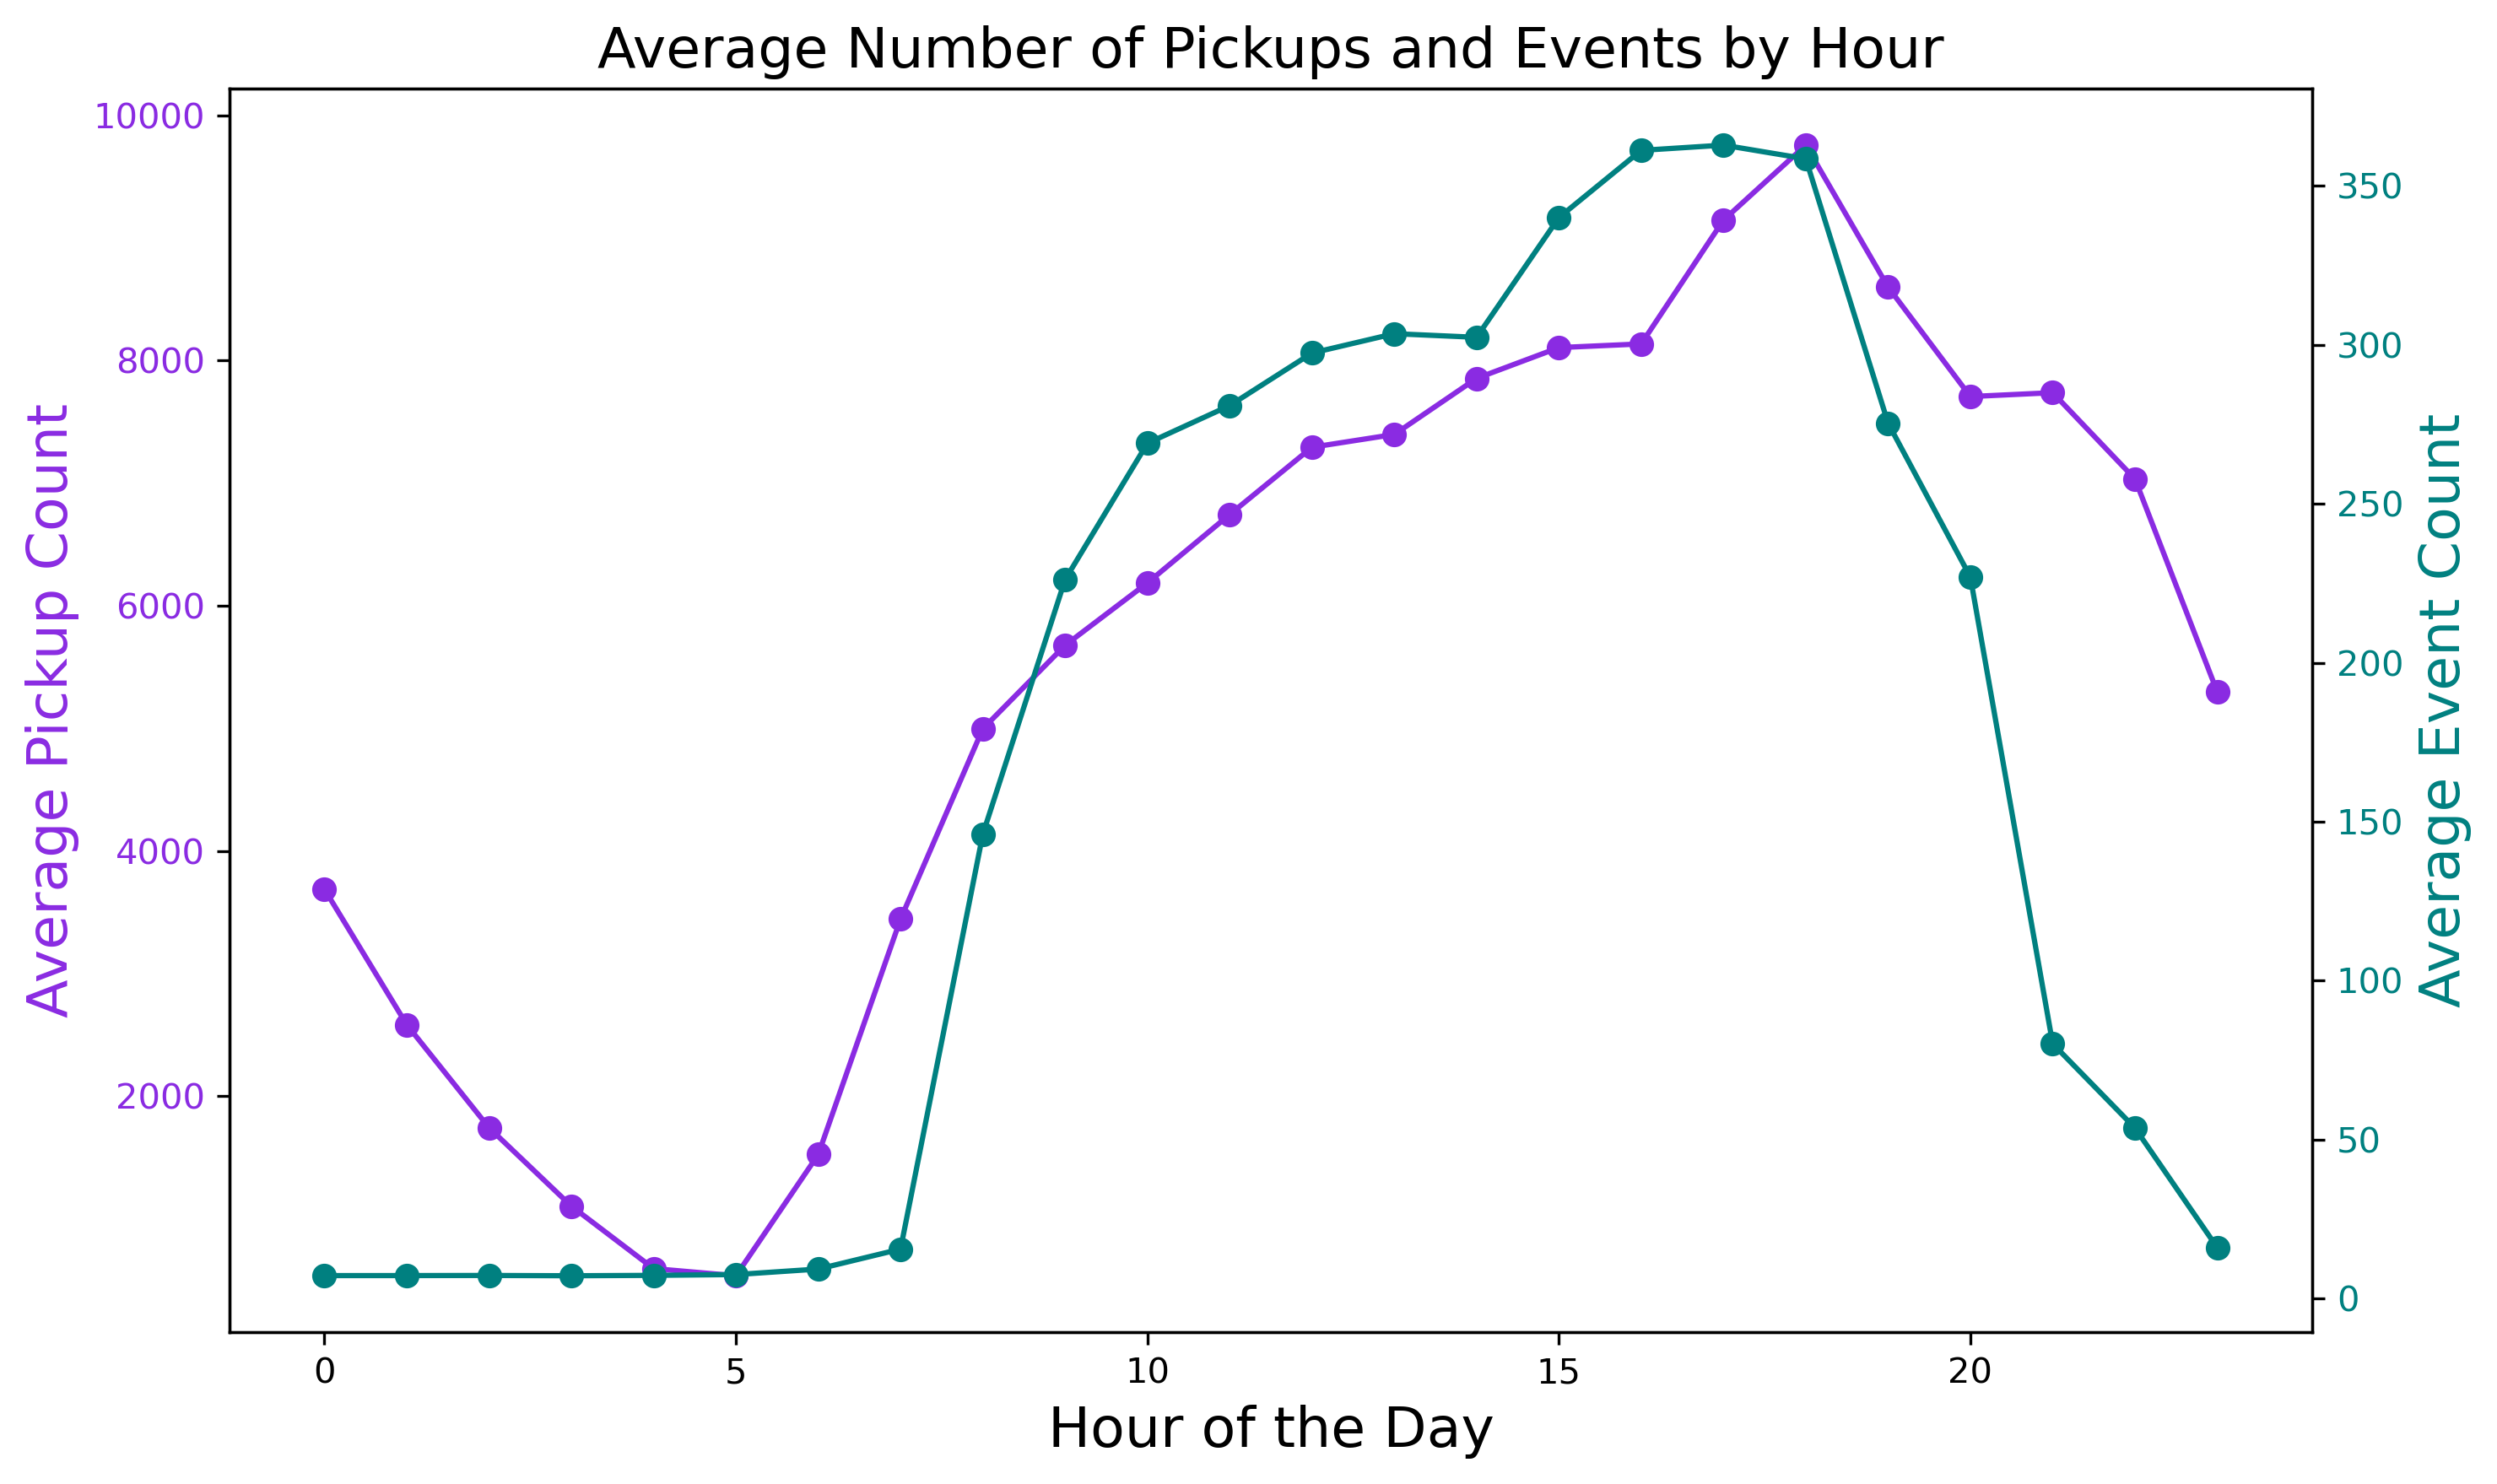
\includegraphics[width=0.5\textwidth]{plots/average_events_pu_hour.png}
    \centering
    \caption{Average Daily Taxi Pickups and Events per Hour}
    \label{fig:events_vs_pickups}
\end{figure}

\subsection{Relationship Between Events and Weather}
To further aid in the model for predicting the hourly demand of taxis based on events in a particular area, I also decided that including the weather might be of great importance as the weather is also something that can affect the number of events in a day. To show this relation, take a look at Figure \ref{fig:events_vs_weather}. The figure shows a relatively linear relation between the number of events and the average temperature for the day. 

\begin{figure}[h]
    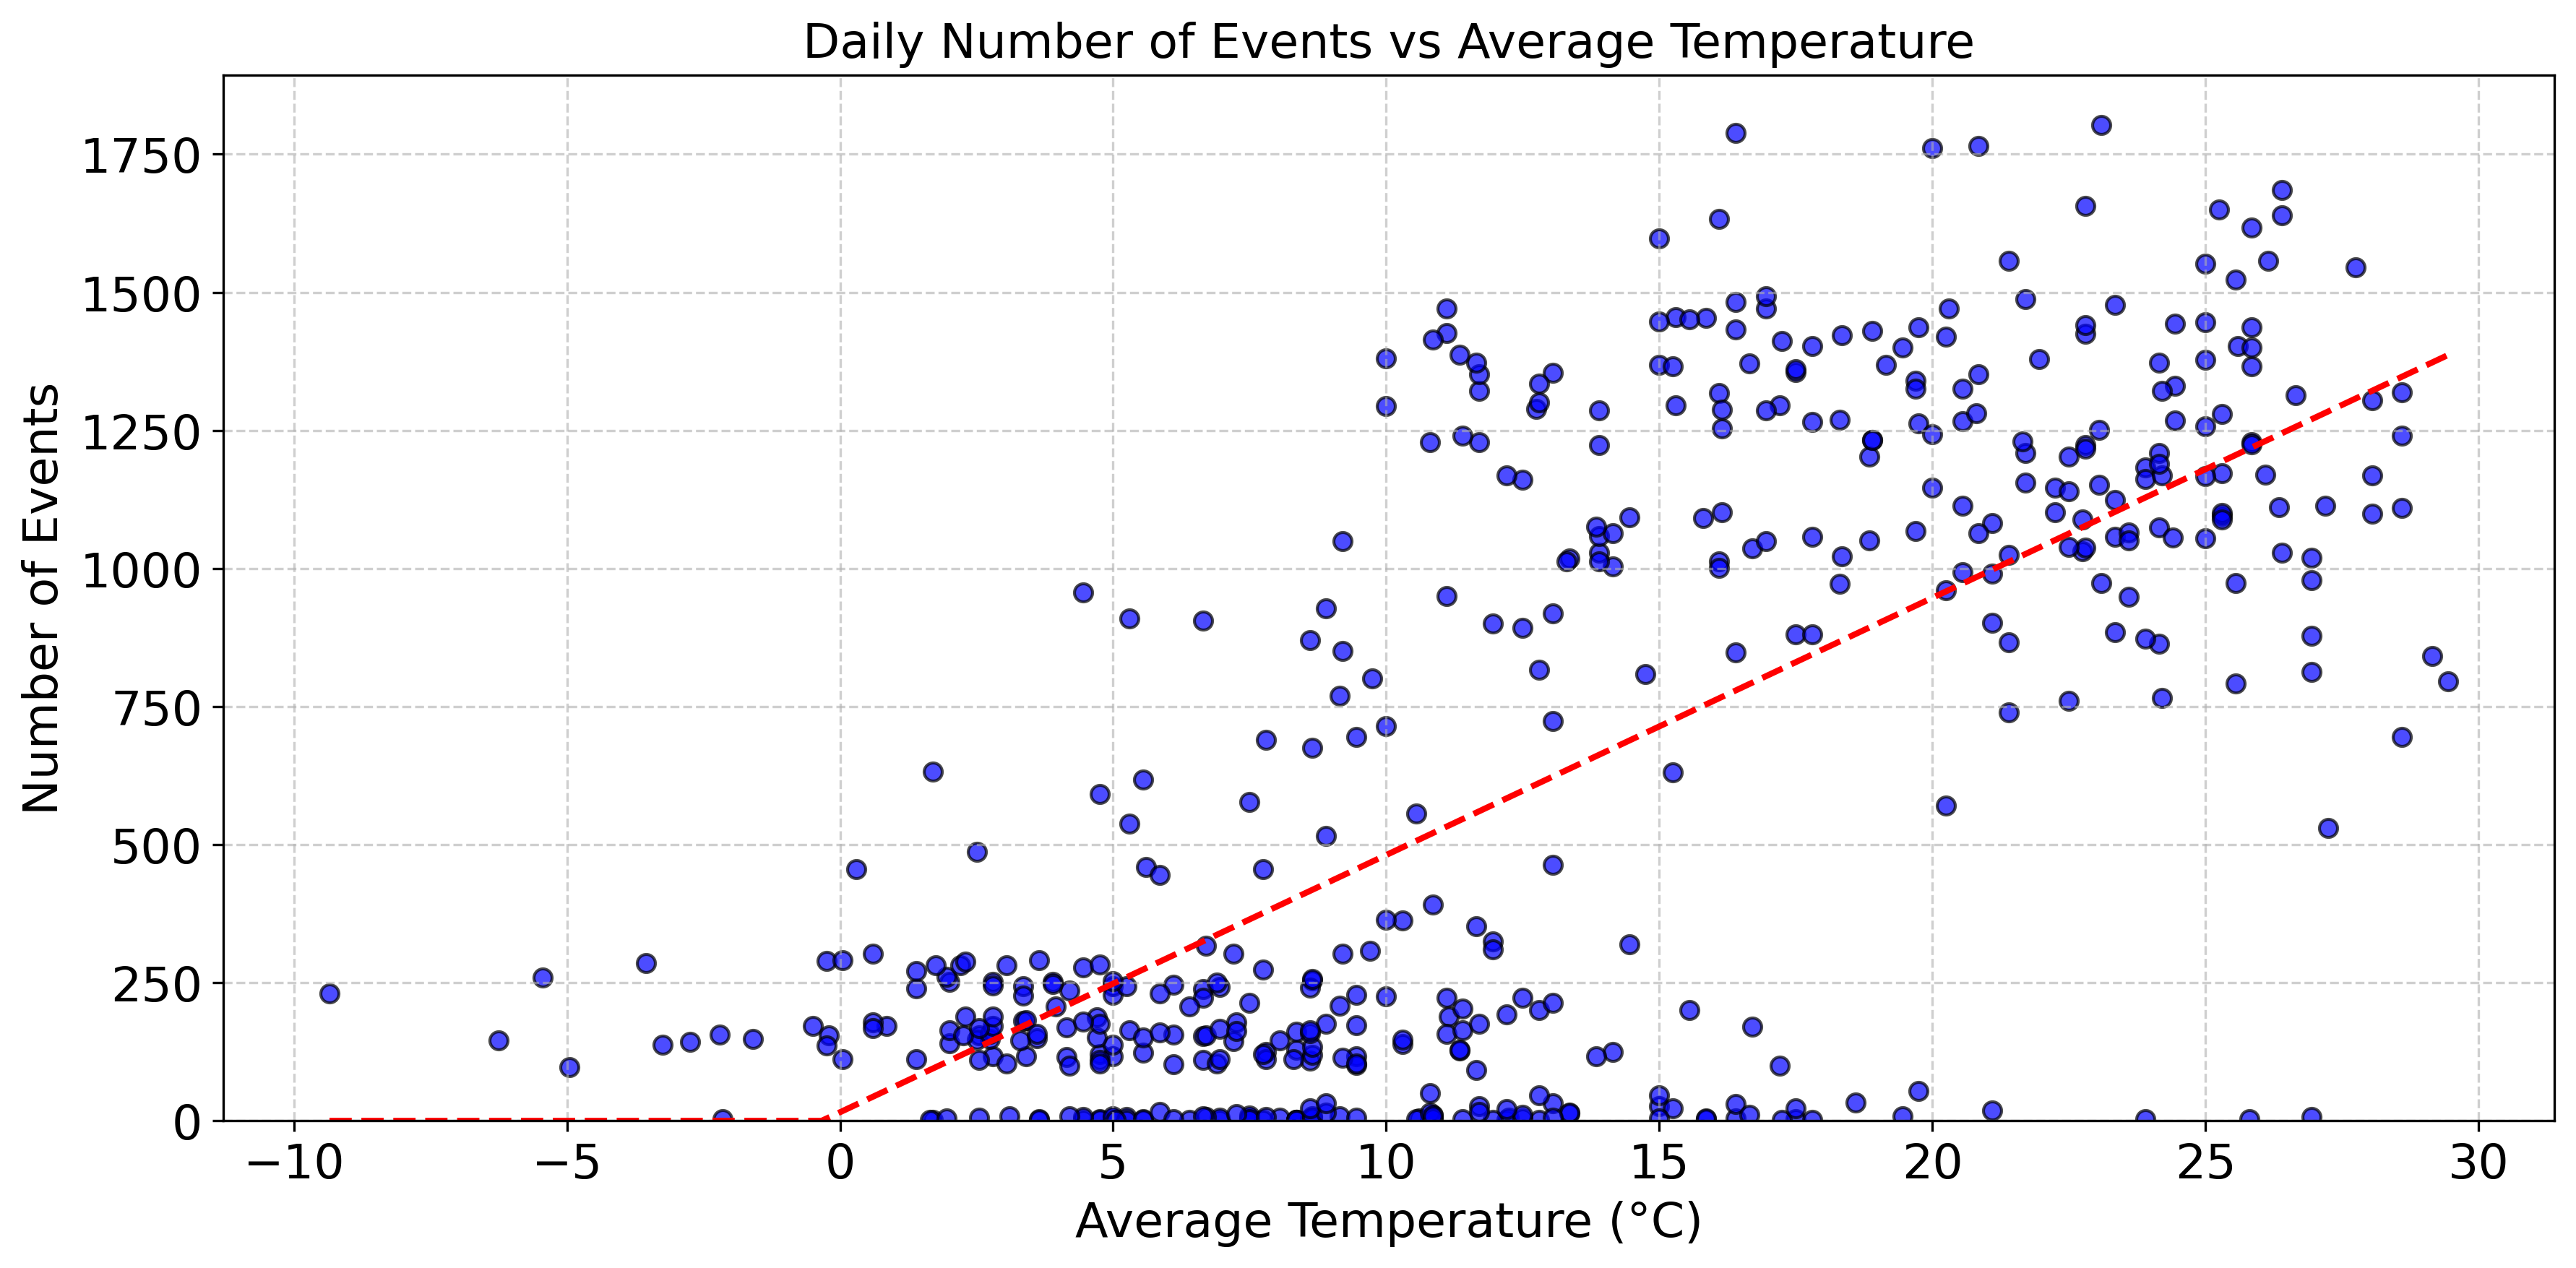
\includegraphics[width=0.5\textwidth]{plots/average_temp_events.png}
    \centering
    \caption{Total Number of Events per Day vs. Average Temperature of the Day}
    \label{fig:events_vs_weather}
\end{figure}

The plot in the figure above shows a clear relationship with fewer events being clustered around at lower temperatures and more events being clustered around the higher average temperatures. As a result, this feature is considered likely to be useful in determining the demand for taxi rides.

\section{Modelling}
\label{sec:modelling}
I decided to fit two different models to try and predict the hourly demand for taxis in NYC. The models are LASSO regression as a baseline model and Gradient Boosting regression to compare.
\subsection{LASSO Regression}
The main goal of choosing the LASSO model as a baseline was to have a somewhat (presumably) better model than a simple linear regression model, as LASSO includes a penalty term, which encourages sparse solutions. Essentially LASSO was chosen over an ordinary least squares method due to its ability to perform both variable selection and regularization, which helps in improving model interpretability and avoids overfitting, especially in a dataset that has many features.
The features used for both models were as follows:
\begin{itemize}
    \item Temporal features: these were extracted from the date and time and left us with the hour, day of the week, and month as the key features
    \item Weather features: as mentioned in the preprocessing section \ref{subsec:weather} of the report, I decided to keep precipitation, snowfall, maximum temperature, minimum temperature, average wind speed, average relative humidity, and other weather conditions such as fog and thunder
    \item Event features: count of events and other geospatial features such as precinct and boroughThis list is the list of features that was used to fit on the models in order to try and predict the demand of taxis hourly for the different locations (precincts in this case)
\end{itemize}

We used these features to fit the models to try and predict the hourly demand of taxis for the different locations (precincts in this case). 
The LASSO model was trained multiple times with different lambda values using cross-validation to identify the optimal lambda value, which we compared with the other model.


\subsection{Gradient Boosting Regression}
The same features were also fit on the gradient boosting regression model to contrast.
A comparison of the performance of the two models is shown in Table \ref{tab:model_comparison} below.

\begin{table}[h]
    \centering
    \begin{tabular}{lcccc}
        \hline
        & \textbf{MSE} & \textbf{$R^2$} & \textbf{RMSE} & \textbf{MAE} \\
        \hline
        \textbf{LASSO Regression} & 4451.16 & -0.1327 & 66.72 & 51.58 \\
        \textbf{Gradient Boosting Regression} & 3592.75 & 0.0858 & 59.93 & 34.71 \\
        \hline
    \end{tabular}
    \caption{Performance Comparison of LASSO and Gradient Boosting Models}
    \label{tab:model_comparison}
\end{table}


From Table \ref{tab:model_comparison}, we can see that the gradient boosting regression model has a slightly better performance when compared to the LASSO regression model. We can also see that the Mean absolute error differs by about 20. 

The actual numbers and prediction comparisons can be seen in  Figure \ref{fig:predictions} below.
\begin{figure}[h]
    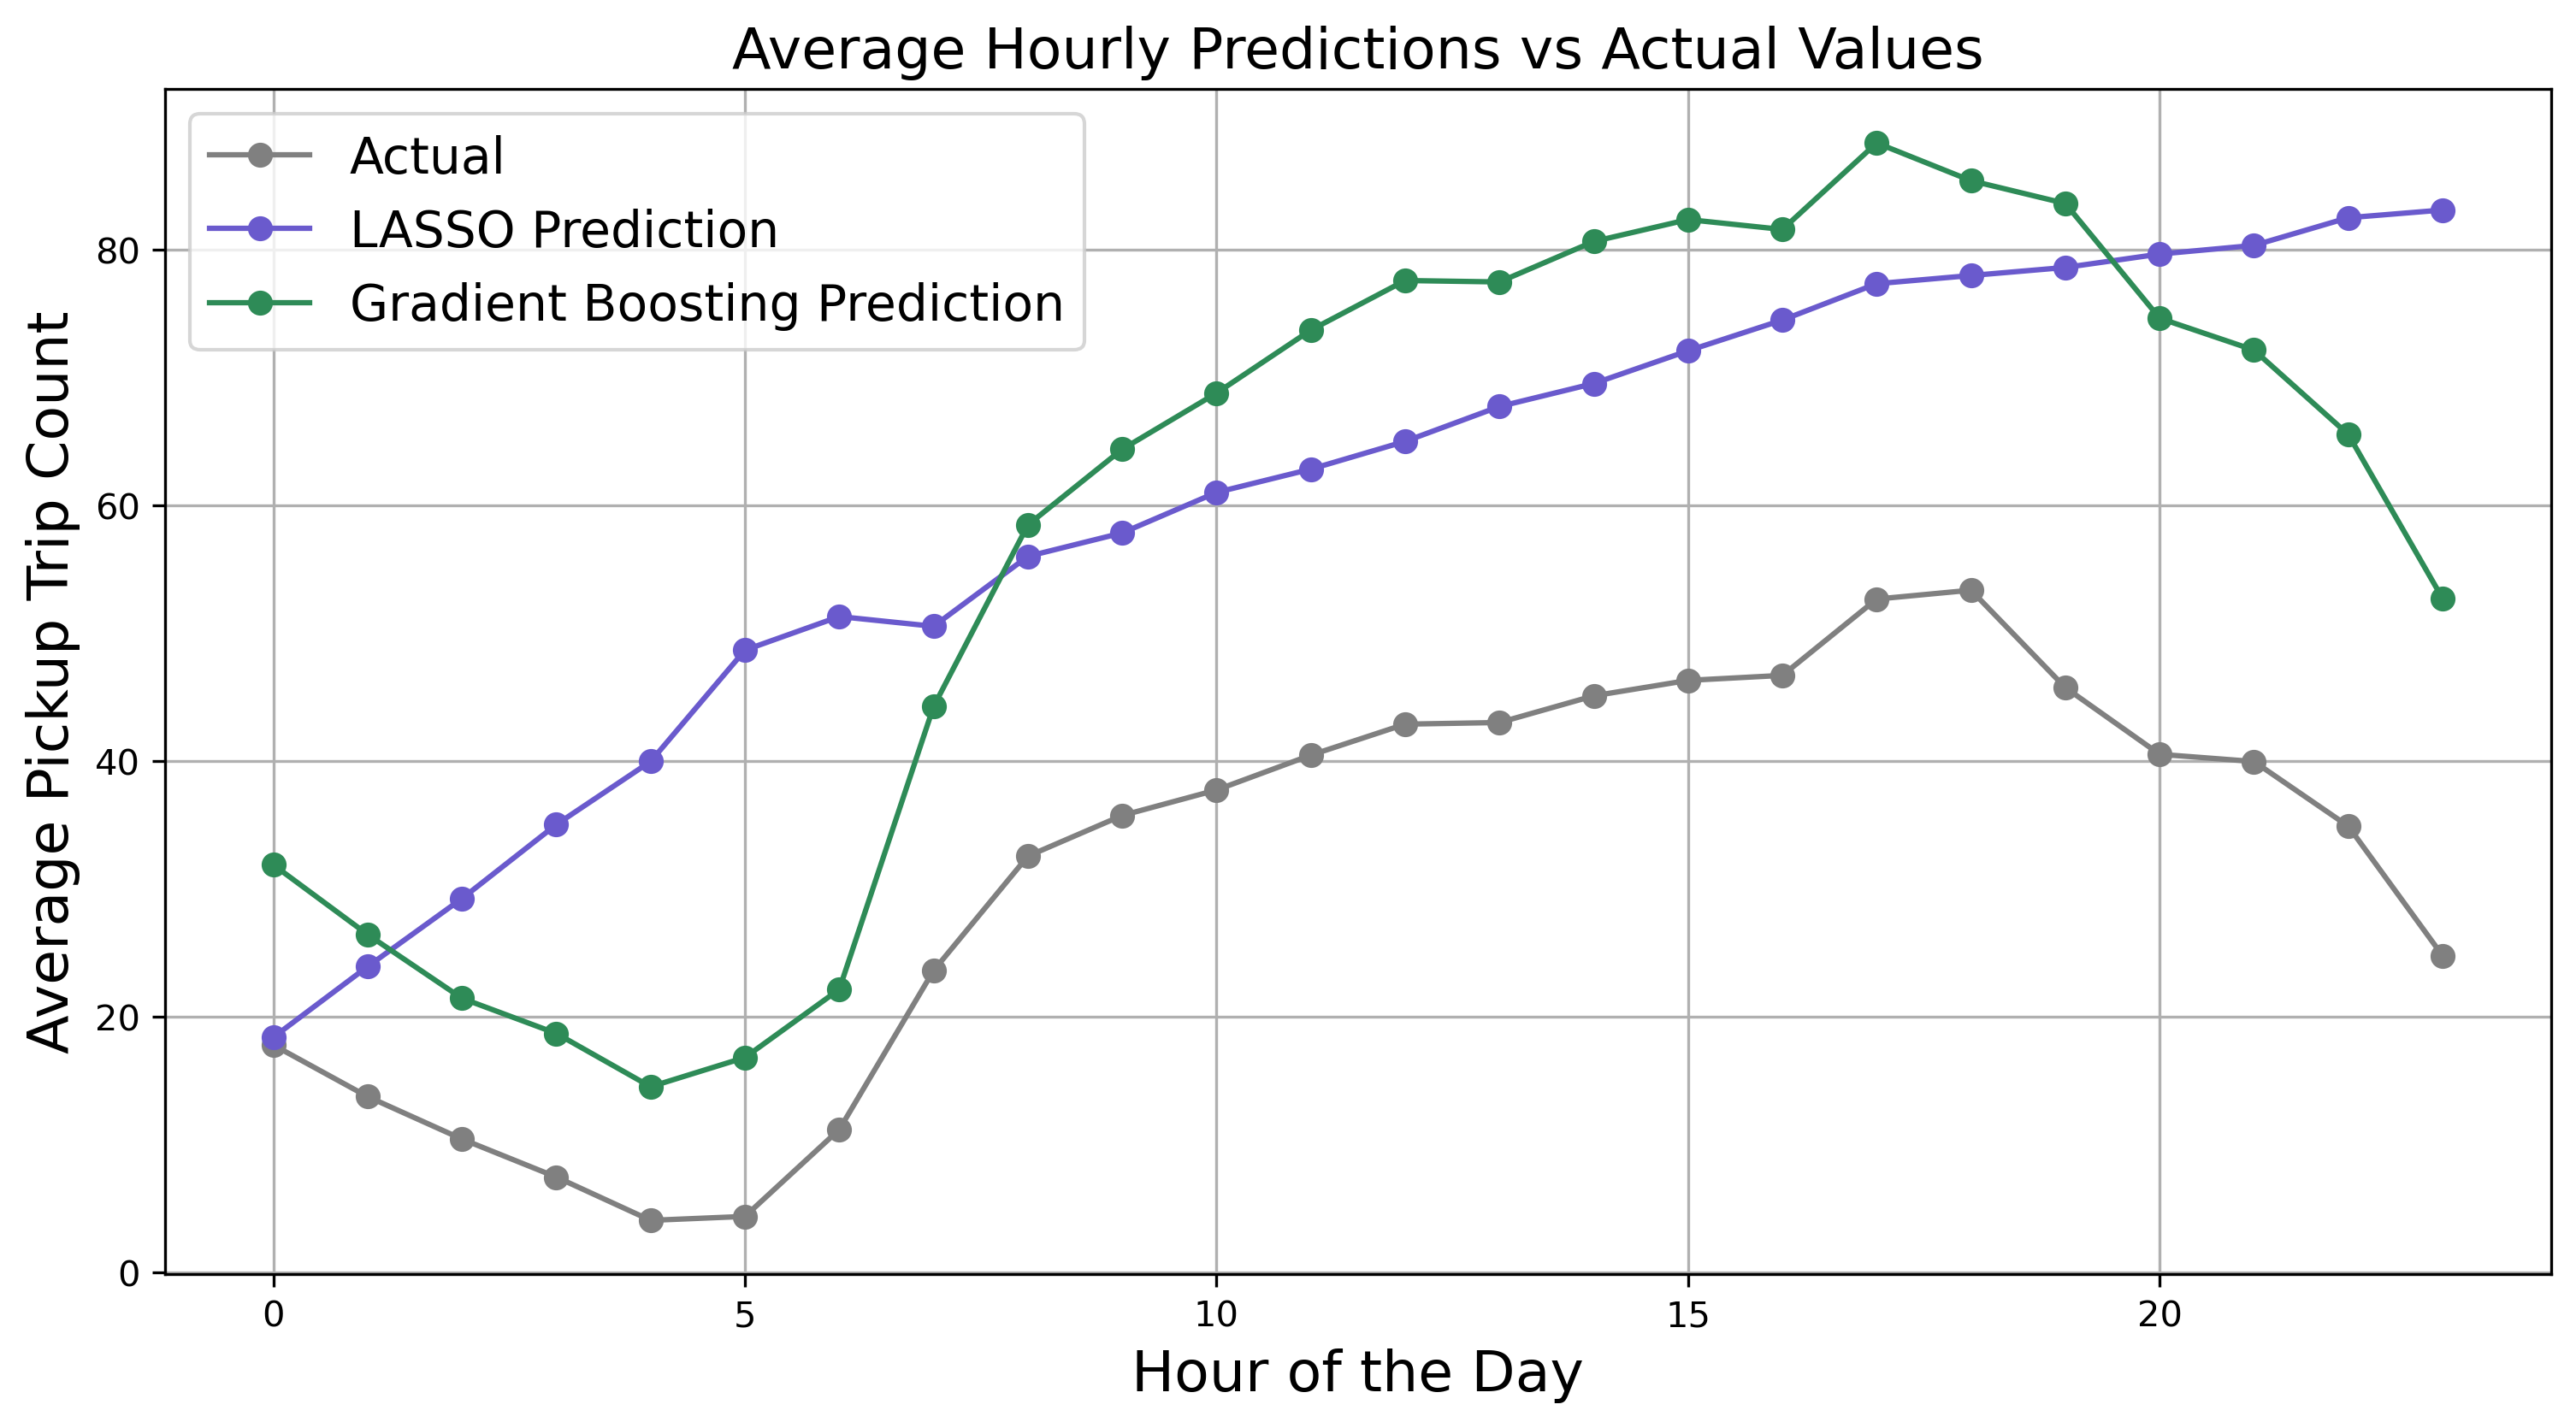
\includegraphics[width=0.5\textwidth]{plots/predictions.png}
    \centering
    \caption{Comparison of Predictions: LASSO vs. Gradient Boosting}
    \label{fig:predictions}
\end{figure}

From Figure \ref{fig:predictions}, we can gauge exactly how the different models fit in terms of the predictions based on the parameters we have in place. 
It can be seen that with the lasso method, the predictions don’t follow the correct pattern and significantly overshoot the numbers when the actual number of pickups is really low. 
Similarly, for the gradient boosting regression model, although it follows a better pattern, it also overshoots the predictions by quite a bit. However, it still seems to perform a little better than lasso. It follows the same pattern as the actual values. There might be some underlying factors that we are unaware of that add to the reasons for this as will be discussed in the following section.

\section{Discussion}
\label{sec:discussion}
As seen from the modeling in Section \ref{sec:modelling}, we do not get the best possible model in this case. This can be due to many things, and here, it seems like the model is overfitting due to having too many features and cannot generalize to the current year. Aside from that, there could be some underlying factors not accurately featured in the model at hand, preventing getting the best prediction for the demand.
From Figure \ref{fig:trips}, we can see that the sheer volume of taxi pickups in 2023 does not follow the same trend in the current year. One speculation here is that people have moved to using ride-share applications instead of hailing taxis, or it could be due to inflation rates, topics we have not looked into.

\begin{figure}[h]
    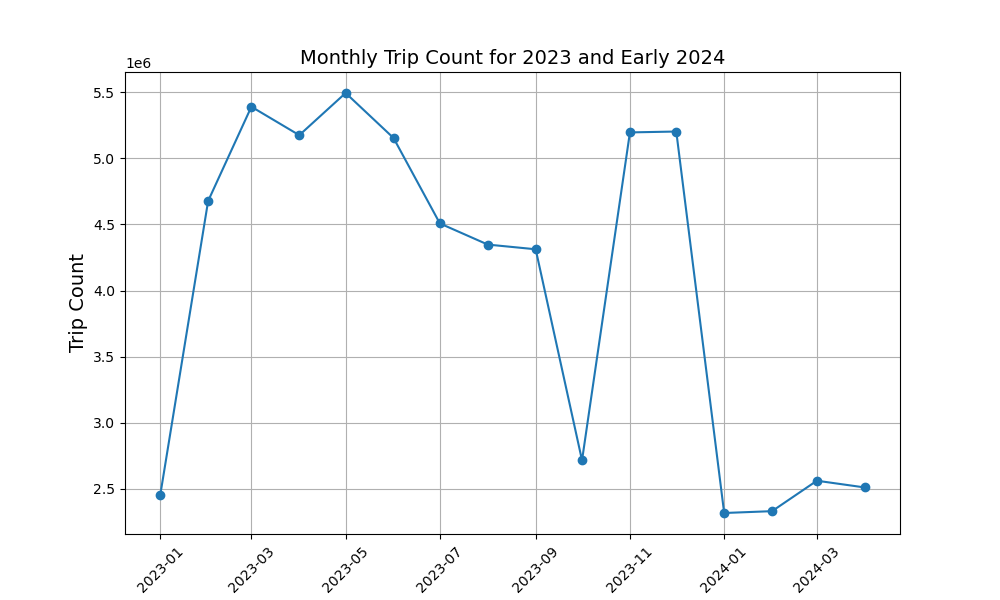
\includegraphics[width=0.5\textwidth]{plots/monthly_trips.png}
    \centering
    \caption{Total Trips per Month}
    \label{fig:trips}
\end{figure}

We could get a better model with better feature creation and selection, but that had limitations due to time and complexity constraints. There might have been some events for the previous year that we might have overlooked and had to remove to try and get more accurate. 
In terms of limitations, a random forest regression model was considered, which might have performed better. However, due to memory constraints on the device used for this project, it was not feasible to implement it with the current number of features. Additionally, running grid search cross-validation for hyperparameter tuning posed a significant risk of overwhelming the device's capabilities, so it was ultimately avoided.
Another limitation of this study is the probably absence of real-time data on traffic. That could likely be an indicator on whether people would hail a taxi or not. 


\section{Recommendations}
One recommendation to the taxi dispatch companies and drivers would be to prioritize Manhattan as a pickup spot, especially from 4 pm to 7 pm. This will help meet the peak demand and also reduce idle time for the drivers, considering the commuter traffic and evening events

Another recommendation would be to provide the drivers with real-time information about the weather and permitted events. For the night owls, an example would be concerts, as they tend to finish late, and the number of pickups is relatively high for odd hours when it's not safe enough to walk around. This can enhance efficiency and guide taxi drivers to locations where people might want to hail a taxi.

\section{Conclusion}
The report focused on predicting hourly demand for taxi rides based on the number of events ongoing in a specific area. The data was fit using two regression models, LASSO regression and Gradient Boosting Regression. From the two models, I found that the Gradient boosting model performed significantly better - with a mean absolute error of 34. LASSO regression, on the other hand, had a mean absolute error of around 50 due to the model overfitting. Essentially, we found that the events and weather can have an effect on the demand for taxis.

Future research can be done of the impact of ride-share services on the demand for taxis, as well as looking into economic factors like inflation. Additionally, further enhancements to the features engineering and selection, along with looking into more robust models might result in better predictions overall. Aside from that, real-time traffic data could also be introduced to get a better view into the demand. 

\clearpage

% BEGIN REFERENCES SECTION
\printbibliography

\end{document}
